
%%%%%%%%%%%%%%%%%%%%%%%%%%%%%%%%%%%%%%%%%%%%%%%%%%%%%%%%%%
\chapter{Related Work}
\label{chapter_related_work}
%%%%%%%%%%%%%%%%%%%%%%%%%%%%%%%%%%%%%%%%%%%%%%%%%%%%%%%%%%

\begin{figure}
\centering
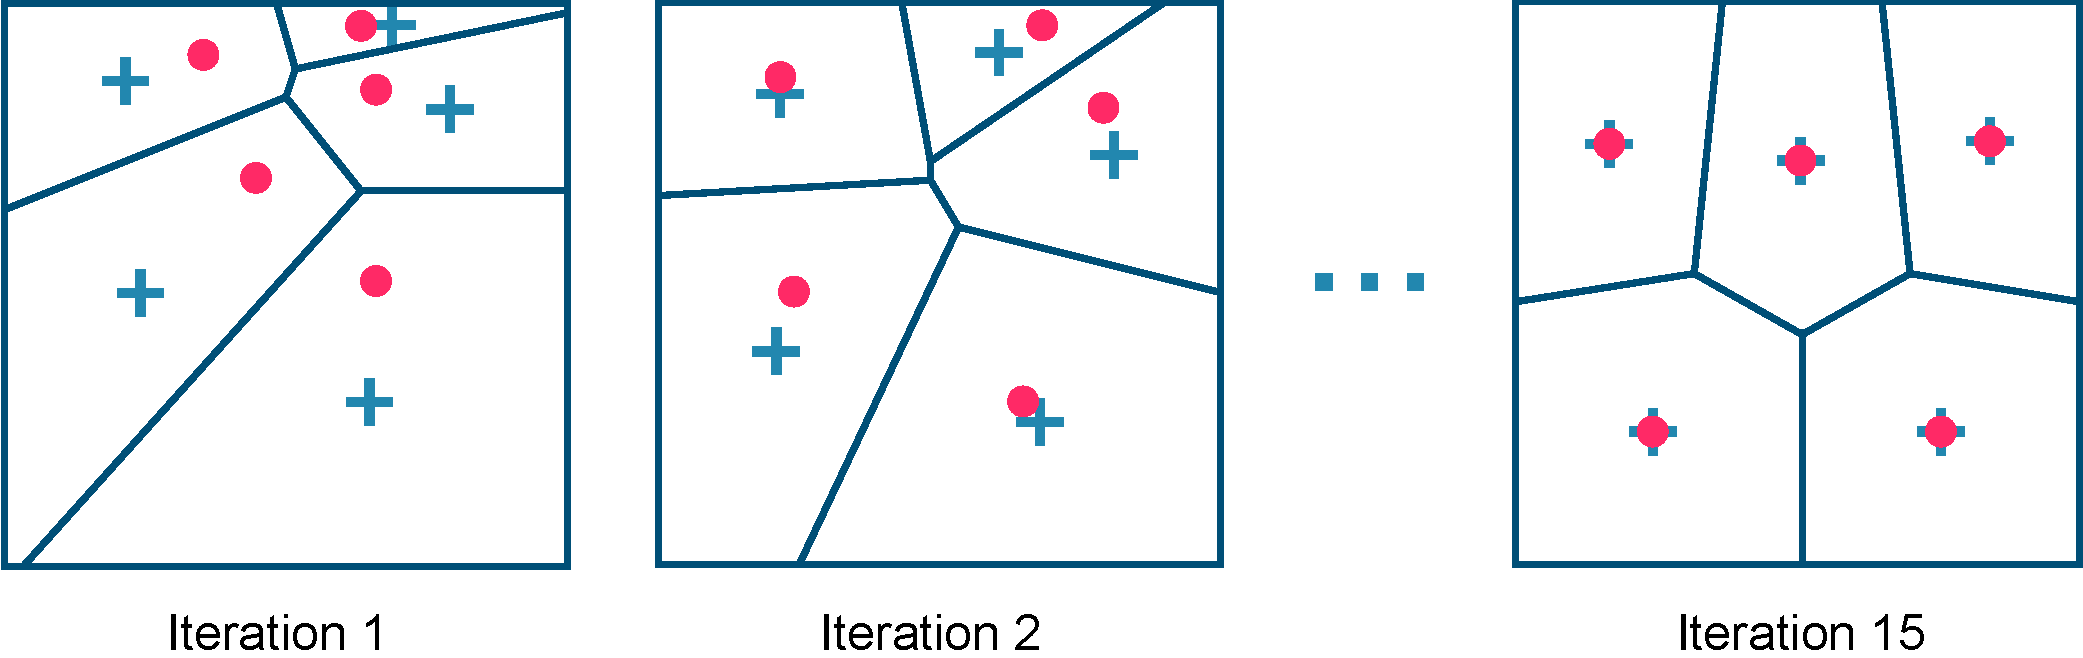
\includegraphics[width=1.0\textwidth]{figures/related/lloyds_method.pdf} 
\caption[An illustration of Lloyd's method.]
{\label{fig_lloyds_method} 
\newtext
{
An illustration of point-based Lloyd's method.
A Voronoi diagram is generated from the input point elements (drawn as red dots).
We then move the point elements to the centroids of Voronoi cells (drawn as plus signs).
The process is repeated until convergence, producing a centroidal Voronoi diagram.
Figure source is Wikipedia, drawn by Dominik Moritz under CC0 1.0.
}
}
\end{figure}


\begin{figure}
\centering
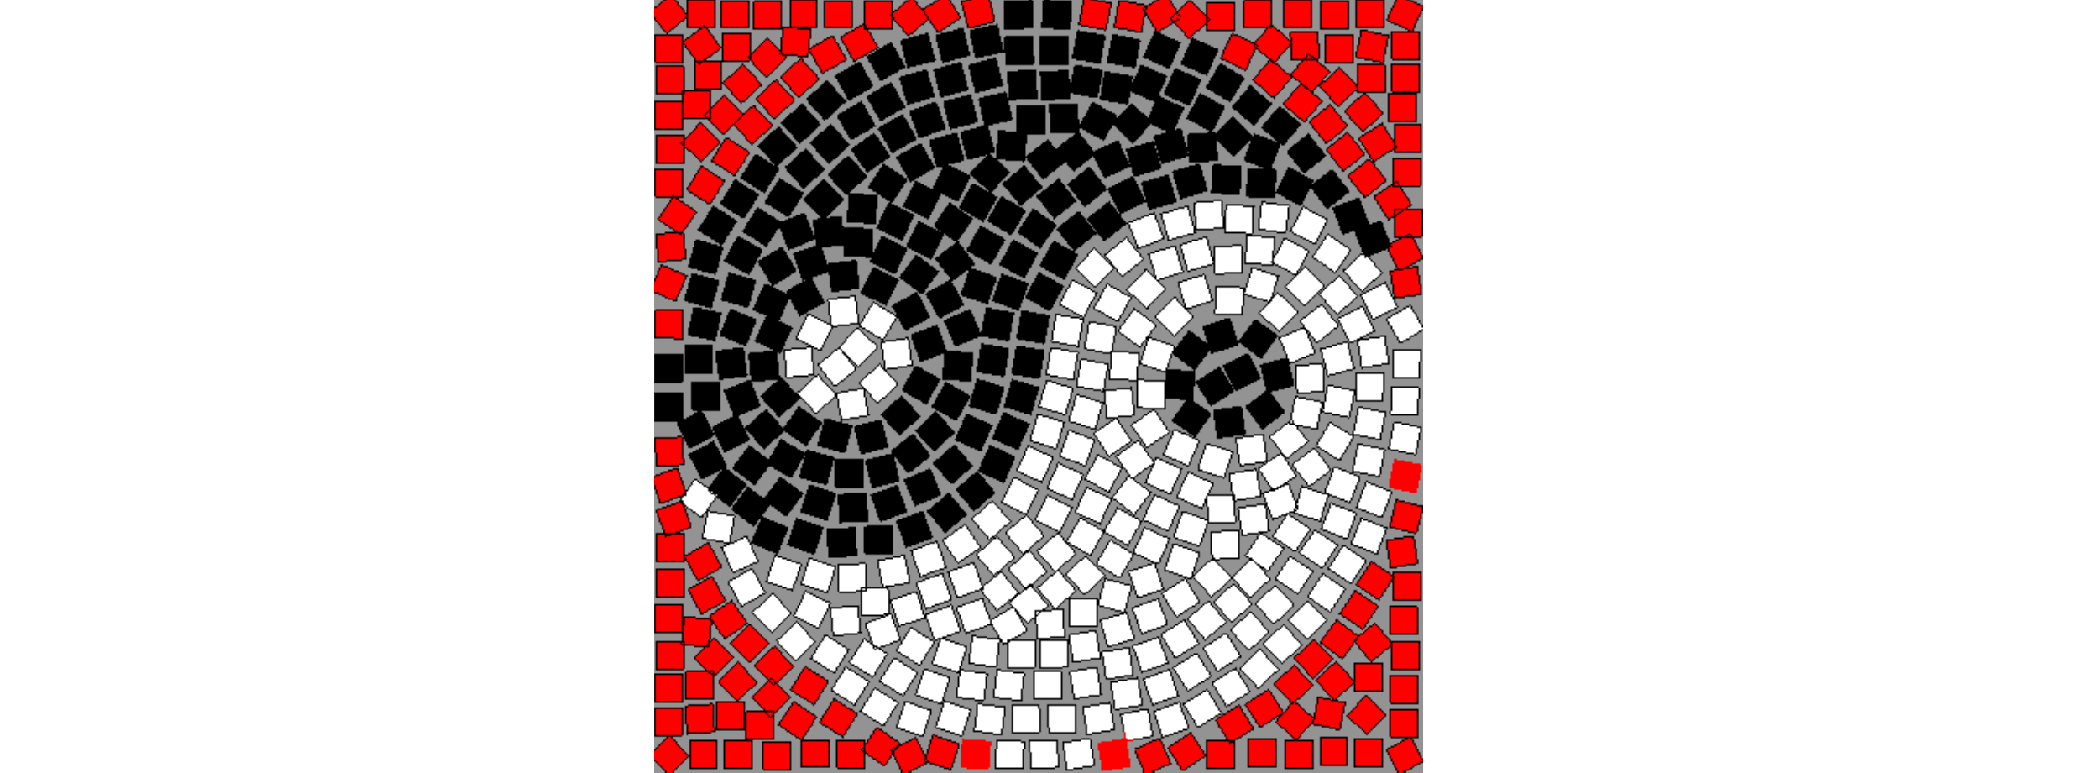
\includegraphics[width=1.0\textwidth]{figures/related/hausner.pdf} 
\caption[Decorative mosaics using Lloyd's method]
{\label{fig_related_hausner} 
\newtext
{
Mosaics of square elements generated using Lloyd's method with Manhattan distance~\cite{Hausner2001}
}
}
\end{figure}





%%%%%%%%%%%%%%%%%%%%%%%%%%%%%%%%%%%%%%%%%%%%%%%%%%%%%%%%%%
\section{2D Packings}
%%%%%%%%%%%%%%%%%%%%%%%%%%%%%%%%%%%%%%%%%%%%%%%%%%%%%%%%%%

%Rigid packing algorithms attempt to distribute elements through rigid transformations.
%These algorithms can be categorized into two groups: iterative methods and data-driven methods.
%Iterative methods start with an initial configuration then they use a variant of Lloyd's method 
%to refine the configuration to an even distribution of elements.
%data-driven methods rely on a shape matching algorithm to find a matching element from
%an element library.
%Some of rigid packing algorithms have an additional step where they 
%correct gaps and overlaps using deformation, the deformation was applied
%locally near edges in a post-processing step after elements
%were frozen in place.

\newtext
{
\textbf{Lloyd's Method:}
An approach to generate a packing is to start with an initial configuration and iteratively refine it using Lloyd's method
to obtain an even distribution of elements. 
%Figure~\ref{fig_lloyds_method} shows an illustration of the simplest example of 
%Lloyd's method that distributes point elements.
Figure~\ref{fig_lloyds_method} shows an illustration of point-based Lloyd's method.
Given $N$ point elements, 
we first compute a \textit{Voronoi diagram} that partitions the plane into $N$ regions such that
all points inside a Voronoi cell are closest to its associated point element.
Lloyd's method moves every point element to the centroid of its Voronoi cell, 
then the Voronoi diagram is recomputed.
The process is repeated until the distribution is even,
that means all the point elements are located at the the centroids of the Voronoi cells.
The final structure is called a \textit{centroidal Voronoi diagram} (CVD).
}

\newtext
{
Secord~\cite{Secord2002} computed a weighted CVD so that the resulting point element distribution
resembles a stippling artwork.
His method incorporates the gradient of an input image into the centroid calculation, 
attracting point elements to low-intensity regions.
%Secord~\cite{Secord2002} distributed point elements by computing a weighted centroidal Voronoi diagram.
%The gradient of an input image is incorporated into the centroid calculation, 
%attracting point elements to low-intensity regions so that
%the final point distribution resembles a stippling drawing.
}


\newtext
{
A standard CVD is generated using Euclidean distance metric, but it can be replaced
to manipulate the shapes of Voronoi cells.
Hausner~\cite{Hausner2001} used this idea to distribute square elements into a container 
region, simulating the appearance of traditional mosaics (Figure~\ref{fig_related_hausner}). 
This can be achieved by using Manhattan distance metric so that Voronoi cells resemble squares instead of hexagons,
each is then replaced with a square element.
In addition, Hausner incorporated a vector field to modify the orientation of the metric
so that the square elements can be rotated. 
However, Hausner's approach is only suitable for square elements as
more complicated shapes such as long rectangles would have severe overlaps.
More recently, Javid et al.~\cite{Javid2019} constructed a metric that 
incorporates a spatial distance, a color distance, and an elongation factor. Their resulting
Voronoi cells have elongated shapes, resembling pebble-like mosaics.}

\newtext
{Hiller et al.~\cite{Hiller2003} improved upon the Lloyd's method to generate \textit{centroidal area Voronoi diagram} (CAVD),
a variant of CVD that is a distribution of simple polygonal elements.
This new extension computes the main inertia axis for each Voronoi cell so that 
its element can be rotated to get better alignment with the Voronoi cell boundary.
In follow up work, Smith et al.~\cite{Smith2005} generated temporally coherent animated mosaics by utilizing CAVD.
Dalal et al.~\cite{Dalal2006} used an FFT-based image correlation to reposition
and rotate elements so that they achieve the best alignments with their Voronoi cell boundaries, 
which could be seen as making more effective use of negative
space, and permitting non-convex elements to interlock more than they did in
earlier methods.
}

\newtext
{
\textbf{Data-Driven Method:} 
A different approach to generate packings is to use a shape matching algorithm (Figure~\ref{fig_related_jim_pad}).
This is usually done by placing an element one by one until the container area is filled.
For each step, a shape matching algorithm selects an 
element that has the best compatibility with the previously placed elements or the container boundary.
Jigsaw Image Mosaics~\cite{Kim2002} uses a geometric hashing to find
a compatible element. JIM places elements using a greedy approach, but is able to backtrack 
if a previous configuration is more optimal.
Pyramid of Arclength Descriptor~\cite{Kwan2016} is
a partial shape matching algorithm that can match
subsets of element boundaries.
}

\newtext
{
It is also possible to initially partition the container into smaller segments
then independently replace each segment with a matching element.
This is desirable if the container has colors or salient parts that need to be emphasized.
Huang et al.~\cite{Huang2011} produced Arcimboldo-like collages
by arranging cutout images collected from the internet.
Their container is a larger cutout image which is partitioned into parts
using an image segmentation algorithm.
Each part is then replaced with a smaller cutout image that has a similar shape and color.
}

\newtext
{
All these data-driven methods require an element library that is big enough,
the more elements in the library will increase their chance to find a compatible element boundary.
However, bigger database means increased computational time and
collecting a large number of elements is also not always feasible.
%for example, if an artist wants to create a packing of a hand-drawn cats,
%they may not want to draw 1000 cats which is tedious and repetitive.
}

\begin{figure}
\centering
\includegraphics[width=1.0\textwidth]{figures/related/jim_pad.pdf} 
\caption[Packings generated by JIM and PAD]
{\label{fig_related_jim_pad} 
\newtext
{
Data-driven methods:
(a) Jigsaw Image Mosaics~\cite{Kim2002}.
(b) Pyramid of Arclength Descriptor~\cite{Kwan2016}. 
}
}
\end{figure}




\begin{figure}
\centering
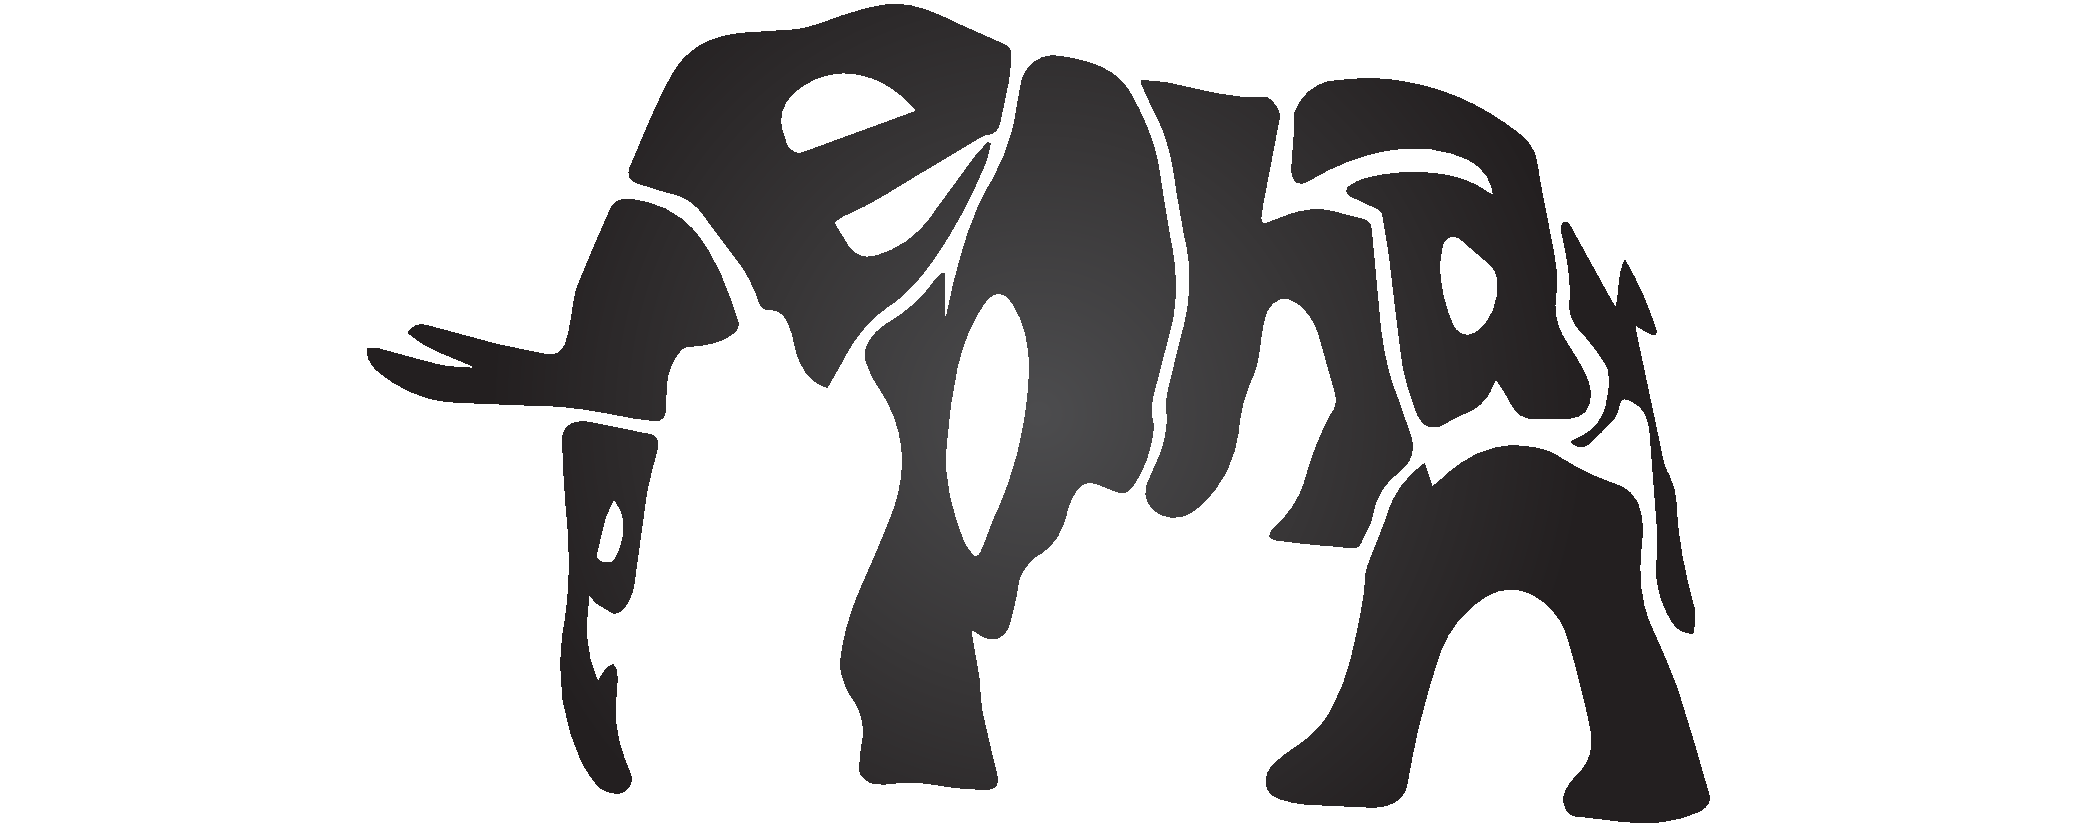
\includegraphics[width=1.0\textwidth]{figures/related/calligraphy.pdf} 
\caption[A calligraphy packing of an ``elephant'']
{\label{fig_calligraphy_packing} 
\newtext
{
A deformation-driven packing of a calligraphic ``elephant''~\cite{Xu2007}.
}
}
\end{figure}

%%%%%%%%%%%%%%%%%%%%%%%%%%%%%%%%%%%%%%%%%%%%%%%%%%%%%%%%%%
%\section{Non-rigid Packing Methods}
%%%%%%%%%%%%%%%%%%%%%%%%%%%%%%%%%%%%%%%%%%%%%%%%%%%%%%%%%%

% need to consult to FLOWPAK for variety
\newtext
{
\textbf{Deformation-Driven Method:}
Instead of finding compatible elements,
a deformation-driven method allows elements to create compatibilities.
As an advantage, a deformation-driven method can rely on a small size element library.
Peng et al.~\cite{Peng2014} computed layouts by packing and deforming
simple polygons and polyominoes, although their method cannot handle more
complicated shapes.
Xu and Kaplan~\cite{Xu2007} and Zou et al.~\cite{Zou2016}
constructed \textit{calligrams} by filling a container with a small
number of deformed letters composing one or two words (Figure~\ref{fig_calligraphy_packing}).  
Their goal was to balance between filling the container and preserving readability.
Abdrashitov et al.~\cite{Abdrashitov2014} developed
a sketch-based interface where an artist can draw curves where square-like elements are placed along it
create a mosaic arrangement.
After the square elements are frozen in place, 
they are deformed to eliminate overlap, to create shape variations, 
and to even out the negative space.  
}




%%%%%%%%%%%%%%%%%%%%%%%%%%%%%%%%%%%%%%%%%%%%%%%%%%%%%%%%%%
\section{Tilings}
%%%%%%%%%%%%%%%%%%%%%%%%%%%%%%%%%%%%%%%%%%%%%%%%%%%%%%%%%%

\newtext
{
As elements reach perfect compatibility, a packing turns to a tiling, see Figure~\ref{fig_related_escherization} for an example.
The element boundaries interlock, leaving no negative space.
Kaplan and Salesin~\cite{Kaplan2000, Kaplan2004} deformed one or two 
input elements into ones that can tile the plane.
%Given an input element $E$ they look for a similar tileable element $T$
%in a parameterized tiling space using simulated annealing.
Given an input element $E$, they performed a search in a parameterized tiling space to find its
deformed variant $T$.
Due to high frequency deformation,
$T$ is often perceptually unrecognizable from its silhouette unless an interior picture is added.
Their method can fail to find $T$ if $E$ has deep concavity, for example, a ``G'' shape.
The tile $T$ also cannot fill a container due to its highly structured boundary.
}

\newtext
{
Lin et al.~\cite{Lin2018} generated ground-reversal compositions that resemble Escher's Sky and Water I,
where elements serve as both positive and negative space depending on the viewer's perception.
%Given two elements $S_1$ and $S_2$, each is copied, deformed, and arranged to interlock each other.
Given two elements $S_1$ and $S_2$, each is placed on the opposite side of a rectangular canvas.
They are then copied, arranged, and deformed to interlock each other.
The farther a copy from the original element, the more deformed it is, 
creating a ``fading effect'', $S_1$ and $S_2$ spatially fade to nothingness.
This work is data-driven, the user needs to provide $S_1$, 
and the method tries to find a compatible element $S_2$ from a library.
%Given two elements $S_1$ and $S_2$, each is placed on the opposite side of a rectangular canvas,
%they are then copied, deformed, and arranged in rows.  
%The farther a copy from the original element, the more deformed it is. 
%creating a ``fading effect'', $S_1$ and $S_2$ spatially transition to ``nothingness''.
%The gradual deformation also allows the copies perfectly interlock each other.
}



\begin{figure}[t]
\centering
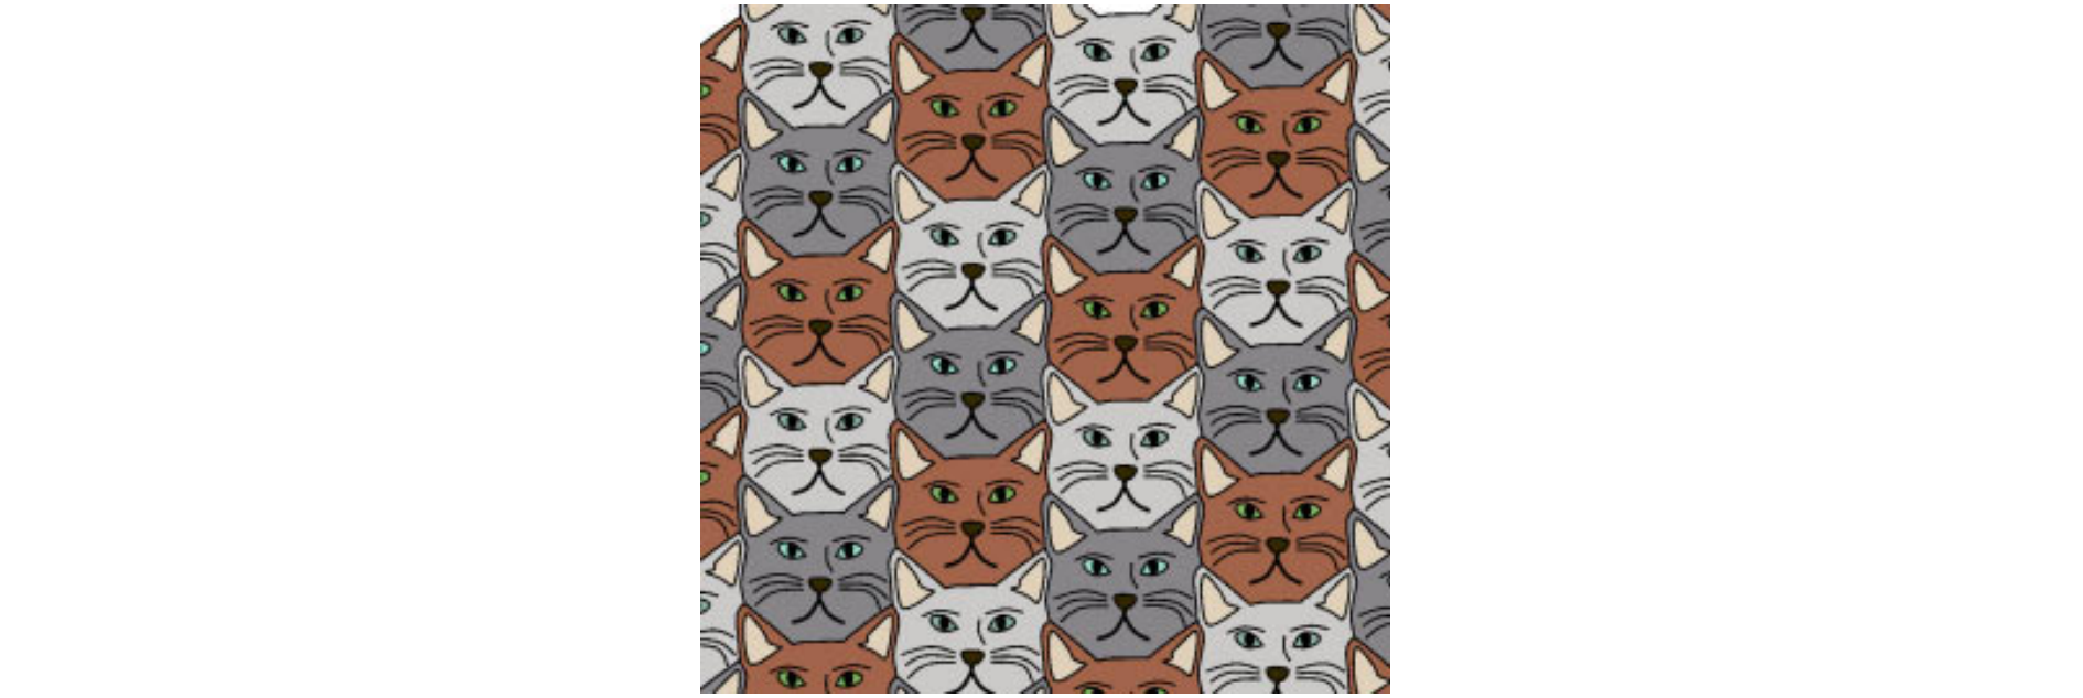
\includegraphics[width=1.0\textwidth]{figures/related/escherization.pdf} 
\caption[A tiling of cats]
{\label{fig_related_escherization} 
\newtext
{
A tiling of cats~\cite{Kaplan2000}, elements perfectly interlock each other and the arrangement does not have negative space. 
}
}
\end{figure}

%%%%%%%%%%%%%%%%%%%%%%%%%%%%%%%%%%%%%%%%%%%%%%%%%%%%%%%%%%
\section{Discrete Texture Synthesis}
%%%%%%%%%%%%%%%%%%%%%%%%%%%%%%%%%%%%%%%%%%%%%%%%%%%%%%%%%%

\newtext
{
Some past work has sought to adapt example-based texture synthesis methods
from raster images to vector graphics, producing distributions of
rigidly transformed elements that mimic the statistics of an \textit{exemplar}.
An element is represented as a single point, which is adequate for small near-convex elements.
Barla et al.~\cite{Barla2006} and Ijiri et al.~\cite{Ijiri2008} used a growth model that copies small neighborhoods
from the exemplar into a larger output texture.  AlMeraj et al.~\cite{AlMeraj2013}
stamped out copies of the exemplar and discarded overlapping elements.
Hurtut et al.~\cite{Hurtut2009} developed a statistical sampling method based
on multitype point processes.  
Loi et al.~\cite{Loi2017} developed a texture synthesis method that
can specify global arrangements, local arrangements, or a blend of multiple arrangements.
These techniques are all concerned with replicating
the uneven element distribution in the exemplar, without regard for negative space.
}

\newtext
{
For larger concave elements, a single point representation is not enough.
Ma et al. ~\cite{Ma2011} used sample-based representation that
is created by generating a sparse set of points inside an element.
They later distributed these points using a neighborhood metric and an iterative optimization.
Unlike previous work, they were able synthesize textures with long deformable elements, for example, spaghetti.
Ma et al. later extended their work to accept animated elements~\cite{Ma2013}, where
each sample point has a spatial and time position, turning the problem to spacetime texture synthesis.
More recently, Hsu et al.~\cite{Hsu2020} adapted the sample-based representation into an interactive app
where an artist can initially distribute elements by drawing strokes
which are then optimized using a Lloyd-like optimization.
}
%Most discrete texture synthesis method treat a single element
%Ma et al.~\cite{Ma2011} used sample-based element representation 
%Ma et al.~\cite{Ma2011} use sparse point samples to represent an element, which
%give an advantage of distributing 




%%%%%%%%%%%%%%%%%%%%%%%%%%%%%%%%%%%%%%%%%%%%%%%%%%%%%%%%%%
\section{3D Packings}
%%%%%%%%%%%%%%%%%%%%%%%%%%%%%%%%%%%%%%%%%%%%%%%%%%%%%%%%%%
\newtext
{
Collages are arrangements of overlapping elements, similar to
portrait paintings by Giuseppe Arcimboldo.
Gal et al.~\cite{Gal2007B} presented a method for constructing 3D
collages (Figure~\ref{fig_related_gal_zehnder}a).  
They filled a 3D container with overlapping 3D elements using a greedy
approach and a partial shape matching algorithm.
Huang et al.~\cite{Huang2014} designed a method
to generate mechanical collages, such as giant robots.
Theobalt et al.~\cite{Theobalt2007}
developed a method to generate animated 3D collages.
They segmented an animated container
into smaller rigid parts, each is replaced with a matching element.
The final result of animated collage consists of rigid motions of elements.
All these collage methods require a 3D shape database so they are considered as data-driven. 
%Both these collage methods require a 3D shape database so they can be considered as data-driven. 
}

\newtext
{
The cutting and packing problem (C\&P) is defined as cutting a large object into smaller parts 
which are then packed inside a container.
C\&P is popular in manufacturing and 3D printing because
objects can be produced with less waste material and packed into a smaller box.
A good cutting process is critical in C\&P, if it can decompose the input object
into simpler parts, then the packing process can be easier.
Chernov et al.~\cite{Chernov2010} proposed a method to decompose a large object
into smaller phi objects which can be packed more efficiently.
A phi object is defined as a shape whose surface boundaries 
are flat, spherical, cylindrical, or conical.
Vanek et al.~\cite{Vanek2014} introduced PackMerger,
a method to pack thin shells which can be assembled together into
a larger watertight object.
In follow up work, Chen et al.~\cite{Chen2015} introduced Dapper,
a method to cut and pack volumetric printed objects.
}

\newtext
{
In engineering, packings are useful for a number of applications, 
such as product packaging, circuit designs, or mechanical layouts.
This requires elements to be packed without any overlap.
Byholm et al.~\cite{Byholm2009} developed a method
to pack voxelized elements, which are computationally easier for collision detection.
Ma et al.~\cite{Ma2018} proposed a heuristic method to pack triangular meshes.
For an in-depth survey, Cagan et al.~\cite{Cagan2002} discussed a few approaches such as
gradient methods, heuristics, simulated annealing, and genetic algorithms.
}



%%%%%%%%%%%%%%%%%%%%%%%%%%%%%%%%%%%%%%%%%%%%%%%%%%%%%%%%%%
\section{Packings on Surfaces}
%%%%%%%%%%%%%%%%%%%%%%%%%%%%%%%%%%%%%%%%%%%%%%%%%%%%%%%%%%



\newtext
{
Some recent work has explored the elaboration of ornamental
patterns on surfaces, under constraints imposed by fabrication.  
Chen et al.~\cite{Chen2016} developed a method to generate a filigree pattern,
which is an arrangement of decorative thin rod elements on a surface.
Given an initial random configuration of overlapping elements, their method
removes overlaps by either deforming or trimming the rods.
Bian et al.~\cite{Bian2018} used Wang tiles made of element parts to generate filigree patterns.
In similar work, Zehnder et al.~\cite{Zehnder2016} 
proposed a semi-automated tool for deforming ornamental curves to cover a surface (Figure~\ref{fig_related_gal_zehnder}b). 
They started with an initial configuration of scaled down elements
that has no overlaps. They later grew the elements and avoided overlaps using curve deformation.
Mart\'{\i}nez et al.~\cite{Martinez2019} developed a CVD-based method to generate
star-shaped tiling patterns that are printed onto tracery sheets.
Their method works by constructing a star-shaped metric to manipulate the Voronoi cell shapes. 
}

%\makeatletter % brooo
%\setlength{\@fptop}{0pt} % brooo
%\makeatother % brooo
\begin{figure}[h]
\bigskip
\bigskip
\bigskip
\centering
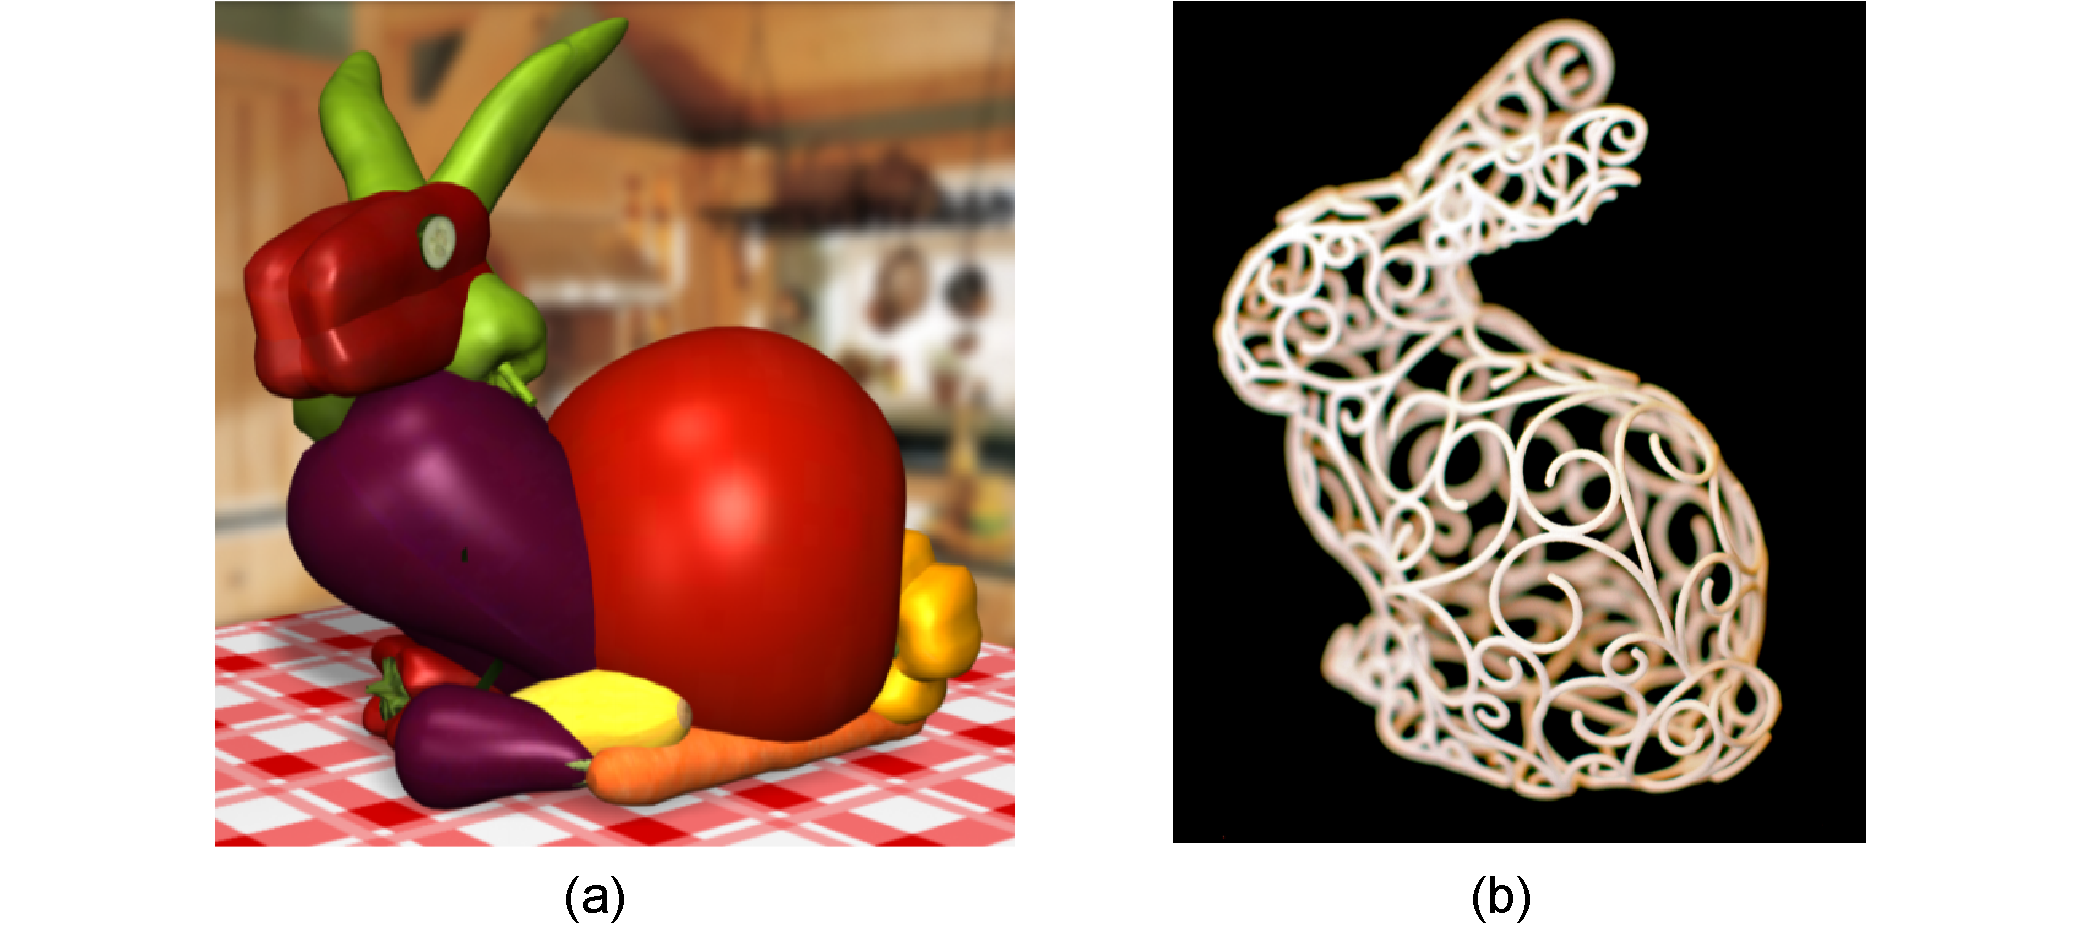
\includegraphics[width=1.0\textwidth]{figures/related/gal_zehnder.pdf} 
\caption[A 3D packing and a packing on a surface]
{\label{fig_related_gal_zehnder} 
\newtext
{
(a) An Arcimboldo-like 3D packing~\cite{Gal2007B}. 
(b) Decorative elements that fill a surface~\cite{Zehnder2016}.
}
}
\end{figure}

